\chapter{Lennard-Jones-Fl�ssigkeit in 2D}
\section{Das Lennard-Jones-Potential}
Nun wird die Simulation auf mehrere Teilchen erweitert. Diese Teilchen befinden sich nicht mehr in einem �u�eren Potential sondern wechselwirken mit sich selbst. Das Potential, das jedes von jedem Teilchen an seiner Position erzeugt wird, wird mit Hilfe des Lennard-Jones-Potentials gen�hert. Da das Lennard-Jones-Potential kugelsymmetrisch ist (keine Richtung wird von den Teilchen bevorzugt) l�sst es sich in Abh�ngigkeit von $r$, dem Abstand zum Teilchen, darstellen. Das Lennard-Jones-Potential ist wie folgt definiert:
\begin{equation}
V(r) = 4\epsilon \left[\left(\frac{\sigma}{r}\right)^{12} - \left(\frac{\sigma}{r}\right)^6 \right]
\end{equation}
Das Minimum des Lennard-Jones-Potentials befindet sich bei $r_c=2^\frac{1}{6}\sigma$. Dies entspricht einer Energie von $E_{min}=V(r_c)=-\epsilon$ Die dazugeh�rige Kraftwirkung erh�lt man durch Differenzieren:
\begin{equation}
F(\vec{r}) = -\nabla V(\vec{r}) = 4\epsilon \left[\left(\frac{\sigma}{r}\right)^{12} - \left(\frac{\sigma}{r}\right)^6 \right]
\end{equation}
$\epsilon$ und $\sigma$ sind charakteristische Gr��en f�r das Lennard-Jones-Potential, wobei $\epsilon$ eine Energie darstellt und $\sigma$ eine L�nge. Dies wird in Abbildung \ref{fig:LJE} und \ref{fig:LJS} dargestellt.
\begin{figure}[htbp]
	\centering
		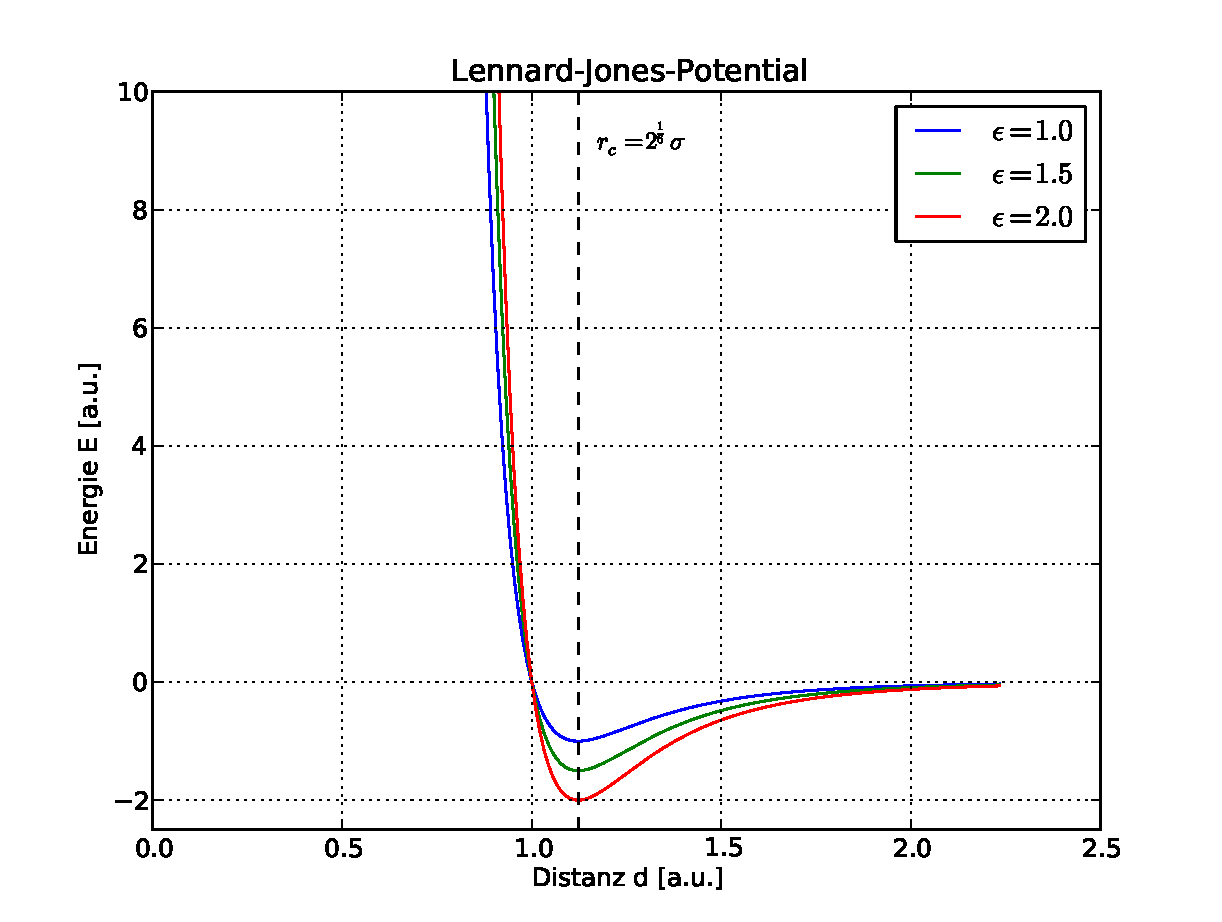
\includegraphics[width=0.70\textwidth]{img/LJE.pdf}
	\caption{Verlauf des Lennard-Jones-Potentials in Abh�ngigkeit der Entfernung. Es zeigt sich, dass $\epsilon$ eine charakteristische Energie darstellt.}
	\label{fig:LJE}
\end{figure}
\begin{figure}[htbp]
	\centering
		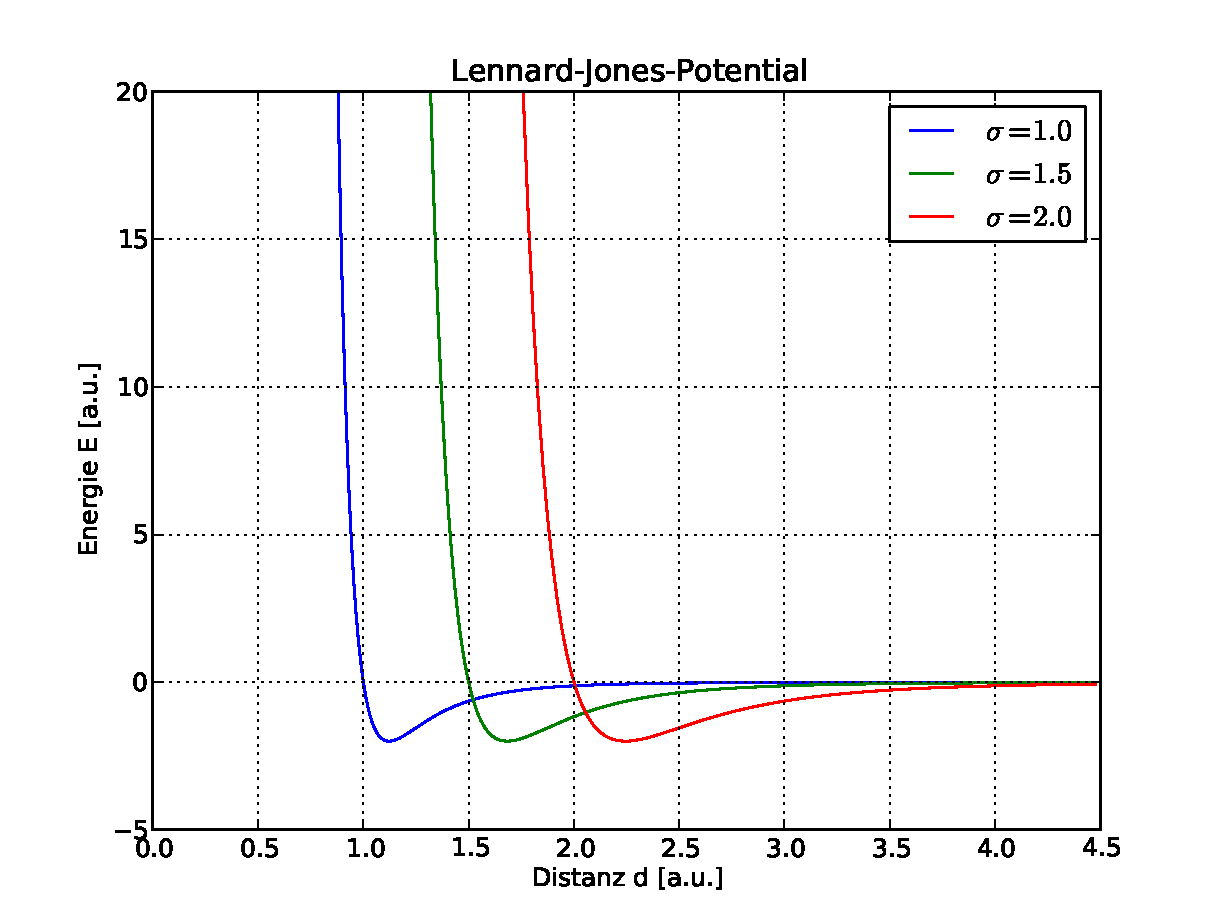
\includegraphics[width=0.70\textwidth]{img/LJS.pdf}
	\caption{Verlauf des Lennard-Jones-Potentials in Abh�ngigkeit der Entfernung. Es zeigt sich, dass $\sigma$ eine charakteristische L�nge darstellt.}
	\label{fig:LJS}
\end{figure}
Wie in den Diagrammen zu erkennen ist, macht es Sinn, alle Einheiten in der Simulation im Bezug auf $\sigma$ und $\epsilon$ anzugeben. Dies wird damit erreicht, dass in der Simulation $\sigma$ und $\epsilon$ gleich 1 gesetzt werden.

\section{Simulation}
Es wird nun eine 2D-Simulation geschrieben, die den zeitlichen Verlauf der Position und der Geschwindigkeit, von $N$ Teilchen ermittelt. Dazu werden die Teilchen zu Beginn auf einem quadratischen Gitter oder einem Dreiecksgitter angeordnet (vgl. \fref{fig:gitter}).
\begin{figure}[htbp]
	\centering
		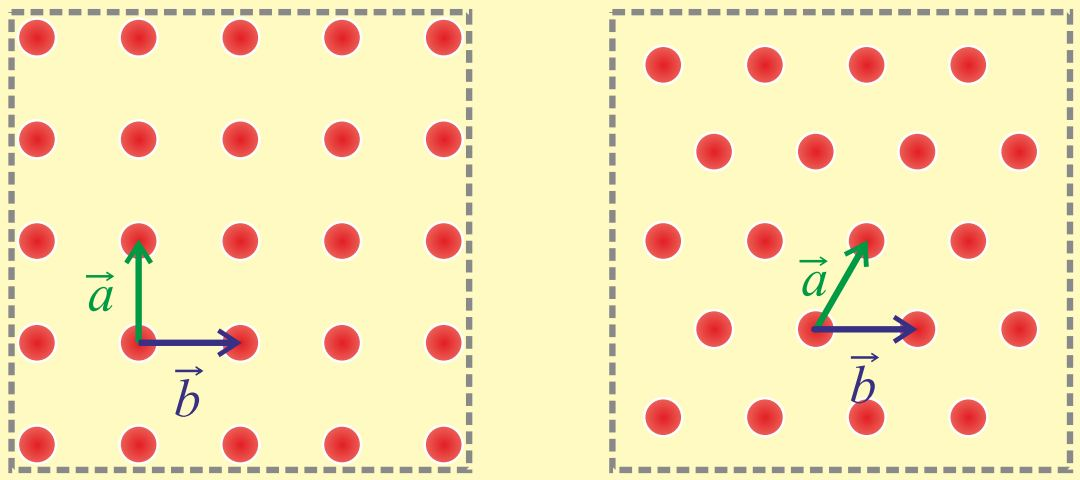
\includegraphics[width=0.80\textwidth]{img/gitter.JPG}
	\caption{Quadratische (links) und dreieckige (rechts) Anordnung der Teilchen zu Beginn der Simulation. Ausschnitt �bernommen aus \cite{schroeder-turk2012}.}
	\label{fig:gitter}
\end{figure}
Es zeigt sich, dass sich die quadratische angeordneten Teilchen sofort in Richtung der Dreiecksstruktur orientieren. Dies l�sst darauf schlie�en, dass die Dreiecksstruktur energetisch g�nstiger ist, als die quadratische. F�r gro�e Zeiten expandiert das System, da die Energie, wie in \fref{chap:HarmOsziNumLsg} gesehen, aufgrund von numerischen Fehlern stetig ansteigt.


\section{Komplexit�t}
Um die Komplexit�t der Simulation zu ermitteln, werden mehrere Simulationen mit unterschiedlicher Teilchenzahl durchgef�hrt. Alle anderen Parameter bleiben dabei unver�ndert. Es wird die Zeit f�r jeden Integrationsschritt gemessen und ein Mittelwert aus 100 Schritten gebildet. Anschlie�end wird an die so gewonnen Daten ein Polynom angefittet, um die Komplexit�t zu bestimmen.
\begin{figure}[h!]
	\centering
		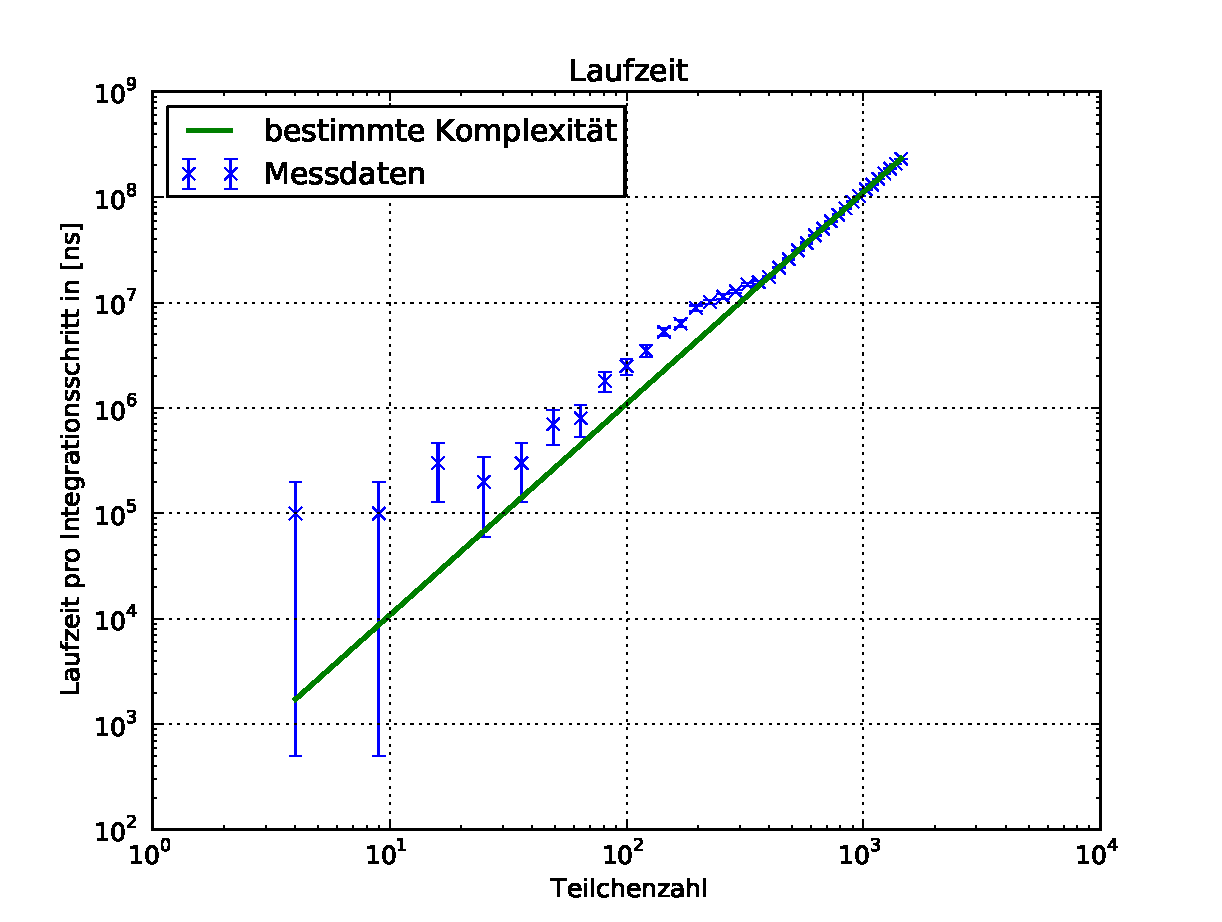
\includegraphics[width=0.70\textwidth]{img/LZ.pdf}
	\caption{Laufzeit in Anh�ngigkeit von der Teilchenzahl mit polynomialen Fit. Es zeigt sich eine $N^2$ Abh�ngigkeit.}
	\label{fig:LZ}
\end{figure}
F�r das Polynom $ax^3+bx^2+cx+d$ ergeben sich folgende Werte: $a=\num{8.65289354e-03}$, $b=\num{9.31841092e+01}$, $c=\num{8.07504705e+03}$ und $d=\num{7.96768647e+05}$. Es zeigt sich, dass die 3. Ordnung vernachl�ssigbar ist. Somit l�sst sich schlie�en, dass das Programm eine Komplexit�t von $O(N^2)$ aufweist.